%
% $RCSfile: command.tex,v $
%
% Copyright (c) 2004. Christian Heller. All rights reserved.
%
% No copying, altering, distribution or any other actions concerning this
% document, except after explicit permission by the author!
% At some later point in time, this document is planned to be put under
% the GNU FDL license. For now, _everything_ is _restricted_ by the author.
%
% http://www.cybop.net
% - Cybernetics Oriented Programming -
%
% http://www.resmedicinae.org
% - Information in Medicine -
%
% @author Christian Heller <christian.heller@tuxtax.de>
%

\paragraph{Command}
\label{command_heading}

The \emph{Command} pattern \cite{gamma1995}, also known as \emph{Action} or
\emph{Transaction}, sometimes also \emph{Signal}, encapsulates a command in
form of an object. That way, operations can get parameterised; they can be put
in a queue, be made undone or traced in a log book. Figure \ref{command_figure}
shows the structure of the pattern.

\begin{figure}[ht]
    \begin{center}
        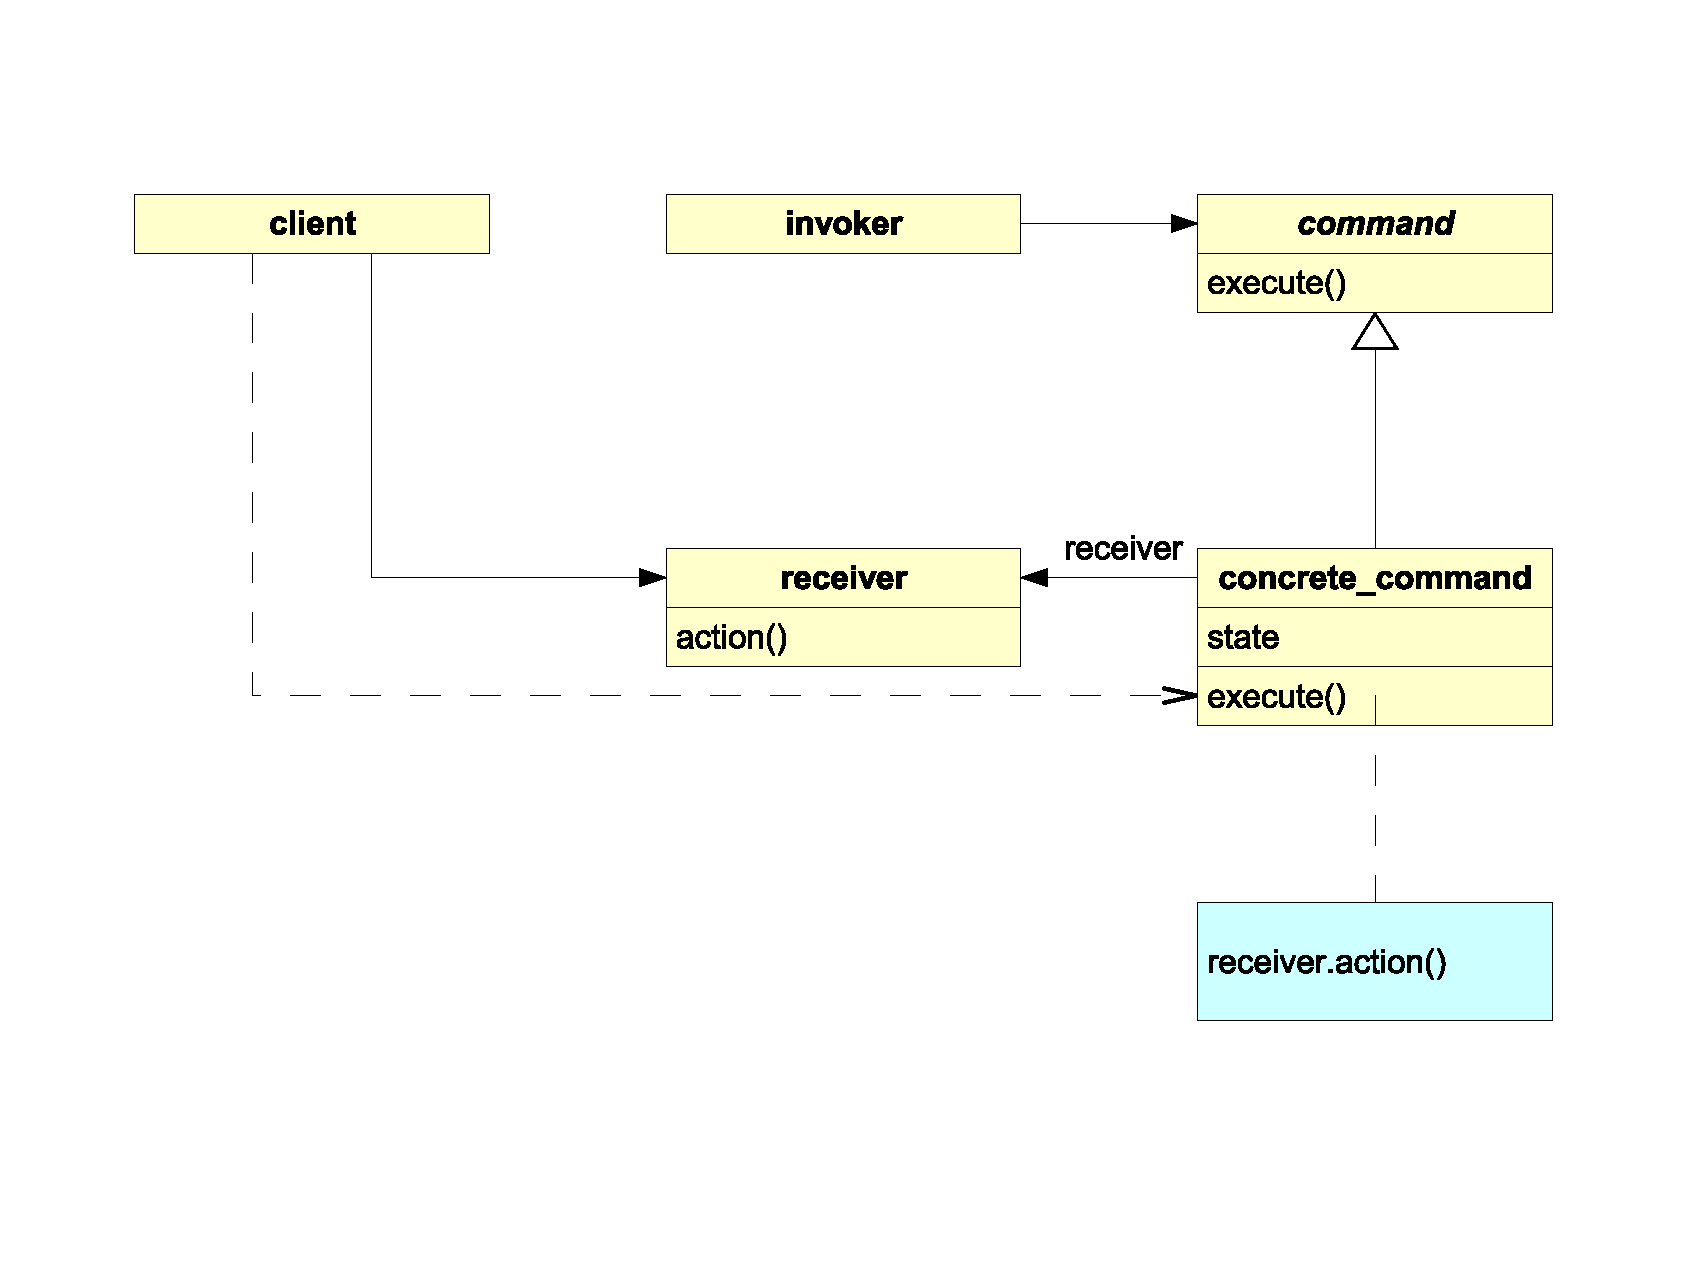
\includegraphics[scale=0.3]{vector/command.eps}
        \caption{Command Pattern}
        \label{command_figure}
    \end{center}
\end{figure}
